\documentclass[preprint,12pt]{elsarticle}
\usepackage{etex}


\makeatletter
\providecommand{\doi}[1]{%
	\begingroup
	\let\bibinfo\@secondoftwo
	\urlstyle{rm}%
	\href{http://dx.doi.org/#1}{%
		doi:\discretionary{}{}{}%
		\nolinkurl{#1}%
	}%
	\endgroup
}
\makeatother
%\usepackage{natbib}
% encoding and languages
\usepackage{hyperref}
\usepackage[utf8]{inputenc}
\usepackage[T1]{fontenc}
\usepackage[ngerman,english]{babel}
\usepackage{wrapfig}
\usepackage{times}
\usepackage{paralist}
\usepackage{graphicx, color}
%\usepackage{subfigure}
\usepackage{subfig}
%\usepackage{subfloat}
\usepackage{booktabs}
\usepackage{caption}
%\usepackage{subcaption}
\usepackage{paralist}
\usepackage{amssymb, amsfonts}
\usepackage{amsmath}
%\usepackage{amsthm}
\usepackage{amsopn}
\newtheorem{myProb}{Problem}
\newtheorem{mythm}{Theorem}

\newtheorem{myproof}{Proof}
\newtheorem{mysketch}{Proof Sketch}
%\usepackage[ruled]{algorithm2e}
%\usepackage[colorinlistoftodos]{todonotes}
%\usepackage{qtree}
\usepackage{tikz, tikz-qtree}
\usepackage[ruled]{algorithm2e}
%\usepackage{Algorithmic}
\usepackage{times}
\usepackage{microtype}
\usepackage{url}
\usepackage{balance}
\let\proof\relax 
\let\endproof\relax
\usepackage{multirow}
\usepackage{relsize}
\usepackage{caption}
\usepackage{color, colortbl}
\usepackage{array, booktabs, ragged2e}
\usepackage{makecell}
\usepackage{tikz}
\usepackage{textpos}

\usepackage{pdflscape}
\newcommand{\RNum}[1]{\uppercase\expandafter{\romannumeral #1\relax}}

\graphicspath{{./Figures/}}

\newcommand{\mypar}[1]{\smallskip\noindent\textbf{#1.}}

\newtheorem{prob}{Problem}


\newtheorem{mydef}{Definition}
%\newtheorem{remark}{Remark}

\newcommand{\todo}[1]{{\textcolor{red}{\bf {#1}}}}

%\newcommand{\mytitle}{Exploiting Software and Hardware Advances  in Optimization Methods for Improved Wind Farm Design}
\newcommand{\mytitle}{Exploiting Hardware and Software Advances 
 for Quadratic Models of Wind Farm Layout Optimization}
%\newcommand{\mytitlerunning}{\mytitle}
%\newcommand{\myauthor}{Arik Senderovich, Eldan Cohen, and J. Christopher Beck}
%\newcommand{\myauthorhyperref}{Arik Senderovich, Eldan Cohen, and J. Christopher Beck}


%\hypersetup{
%    bookmarks=true,        % show bookmarks bar?
%    unicode=true,          % non-latin characters in bookmarks?
%    pdffitwindow=false,    % window fit to page when opened
%    pdfstartview={FitH},   % fits width of the page to the window
%    pdftoolbar=true,       % show acrobat toolbar?
%    pdfmenubar=true,       % show acrobat menu?
%    colorlinks=true,      % false: boxed links; true: color links
%    linkcolor={blue!80!black},       % color of internal links
%    urlcolor={blue!30!black},        % color of external links
%    citecolor={green!60!black},       % color of links to bibliography
%    filecolor=black,       % color of file links
%    pdftitle={\mytitle},           % title
%    pdfauthor={\myauthorhyperref}, % author
%    pdfcreator={\myauthorhyperref} % creator of pdf
%}

\begin{document}
	

\title{\mytitle}
%\subtitle{Extended Abstract}
%\author{}
%\institute{}
%\author{\myauthor}
%\institute{Department of Mechanical and Industrial Engineering, University of Toronto\\
%\email{sariks@mie.utoronto.ca, ecohen@mie.utoronto.ca, jcb@mie.utoronto.ca}}


\author[add1]{Arik Senderovich}

%\ead[url]{https://ischool.utoronto.ca/profile/arik-senderovich/}
\ead{arik.senderovich@utoronto.ca}

\author[add2]{Eldan Cohen}
\ead{ecohen@mie.utoronto.ca}
%\ead[url]{homepageldan}




%\address[1]{}



%\address[2]{40 St. George St., Toronto, Canada}
\author[add2]{Jiachen Zhang}
\ead{jasonzjc@mie.utoronto.ca}

\author[add2]{J. Christopher Beck\corref{cor1}}
\ead{jcb@mie.utoronto.ca}


%\ead[url]{homepageldan}
%\address[3]{}
\address[add1]{Faculty of Information, University of Toronto, 140 St. George St., Toronto, Canada}
\cortext[cor1]{Corresponding author}
\address[add2]{Department of Mechanical and Industrial Engineering, University of Toronto, 40 St. George St., Toronto, Canada}

\begin{abstract} 
%Wind farms play an increasingly important
%role as a source of renewable energy and 
The wind farm layout optimization (WFLO) problem concerns
selecting turbine positions to maximize energy production. While a number of heuristic and exact techniques have been proposed in the literature to solve WFLO, it is natural to model the interaction between turbines as a quadratic objective function as, indeed, has been done in some existing optimization models. Recent advances in optimization hardware and software have both targeted quadratic constraints: commercial mixed integer linear solvers have been extended to quadratic problems and nascent specialized hardware, including quantum computing systems, have focused on solving Quadratic Unconstrained Binary Optimization (QUBO) problems. 
%It is a key problem 
%when designing a new wind farm, as it has a direct influence
%on the amount of the total produced energy. 
%In recent years there have been advances in both software technologies (e.g., the extension of commercial mixed integer linear programming solvers to handle quadratic problems) and nascent hardware development (e.g., quantum computing chips and specialized classical chips) that have relevance for the WFLO problem. In both cases, the advances have 
%Recent years saw 
%advances in software and hardware optimization technologies, such as Gurobi's quadratic solver 
%and Fujitsu's digital annealer (DA), respectively. 
%These technologies create an opportunity to improve 
%over current wind farm optimization solutions
%both in terms of solution quality and solve time. 
%In order to exploit these technologies, 
%we must represent the WFLO problem as 
%a quadratic optimization model. Specifically, in order 
%to apply a software-based optimization
%solution (Gurobi), 
In this paper, we 
introduce two novel quadratic programming models for WFLO: a quadratic constrained optimization problem (QCOP) with binary decision variables and a QUBO.
%Subsequently, we provide the unconstrained counterpart of the QCOP, 
%namely the quadratic unconstrained binary optimization (QUBO), which  
%is the underlying representation for quantum-inspired 
%optimization hardware such as the DA. 
A thorough empirical 
evaluation using a commercial solver and a specialized classical chip for QUBO solving demonstrates the strengths of the two models. 
Our results show that both approaches yield fast and high-quality solutions 
and
improve over existing WFLO solutions. In particular, the QUBO model excels at finding high quality solutions very quickly while the QCOP model is able to find better solutions and provide quality guarantees over a longer run-time.
\end{abstract}
\begin{keyword}
	Wind Farm Layout Optimization (WFLO) \sep Quadratic Programming (QP) \sep Quadratic Unconstrained Binary Optimization (QUBO) \sep Digital Annealer
\end{keyword}

\maketitle 

\section{Introduction}
% Todo
We revisit 
the wind farm layout optimization (WFLO) problem 
that was first considered 
in~\citet{MOSETTI1994105}. 
In WFLO, we aim to place wind turbines 
in a predefined area to maximize 
the total generated power. 
Turbine location decisions    
influence
the
total power production due to  
interference effects, aka wakes, generated by upstream 
turbines. Furthermore, 
there are proximity constraints between turbines
that prevent from turbines to be placed next to each other.
These inter-turbine effects 
are naturally captured using quadratic constraints and objective
functions. Several exact optimization approaches have 
been proposed to solve
the WFLO problem~\cite{turner2014new,Zhang2014}. However, these
approaches represented the quadratic effects and constraints
using linear models that approximate the true dependencies. 

In this work, we introduce two 
novel quadratic WFLO models. The first model 
represents WFLO using a 
quadratic constrained optimization problem (QCOP). 
The QCOP can be solved using state-of-the-art solvers that
specialize in such problems, e.g., Gurobi~\cite{gurobi}. 
Our second model is based on a quadratic unconstrained binary optimization (QUBO) representation of the WFLO 
problem.
This enables the use of specialized optimization hardware tailored to solve
QUBOs. In this paper, we use Fujitsu's digital annealer, a simulated annealing based QUBO solver, to demonstrate the strength
of our approach. The main contributions of this paper are: 
\begin{enumerate} 
\item We propose a novel quadratic modeling framework for WFLO that captures wake 
effects directly through their linear superposition 
without the need for approximations and ad-hoc solutions,
\item We provide the computational complexity of WFLO and show that it is $\mathcal{NP}$-hard, and, 
\item We test our quadratic formulations
on a commerical software-based quadratic solver (Gurobi) and on Fujitsu's digital 
annealer. 
\end{enumerate} Our experiments are focused on the performance of the two approaches
compared to 
existing optimization methods. To this end,
we experiment with 12 standard WFLO benchmark problems (c.f.~\cite{turner2014new})
and show that solving quadratic WFLO models
using Gurobi and the DA
achieves state-of-the-art performance, often outperforming
existing solutions when provided sufficient run-time. Furthermore, we
we observe that the digital 
annealer often provides order of magnitude faster solutions
compared to software-based approaches.

The remainder is structured as follows \todo{adjust structure according to final structure of paper}. 


\section{Background}
\label{sec:related}

We start this section
by presenting the
physical model 
of a wind farm, which we use throughout the paper.
Our wind farm model is based on
the common notation and description 
presented in~\cite{Zhang2014}.  
Subsequently, we provide a literature review of 
existing mathematical
optimization methods for solving WFLO, focusing
on their similarities and differences
compared to our approach.
 
\subsection{The Wind Farm Model}
\begin{figure}[t]
	\centering
	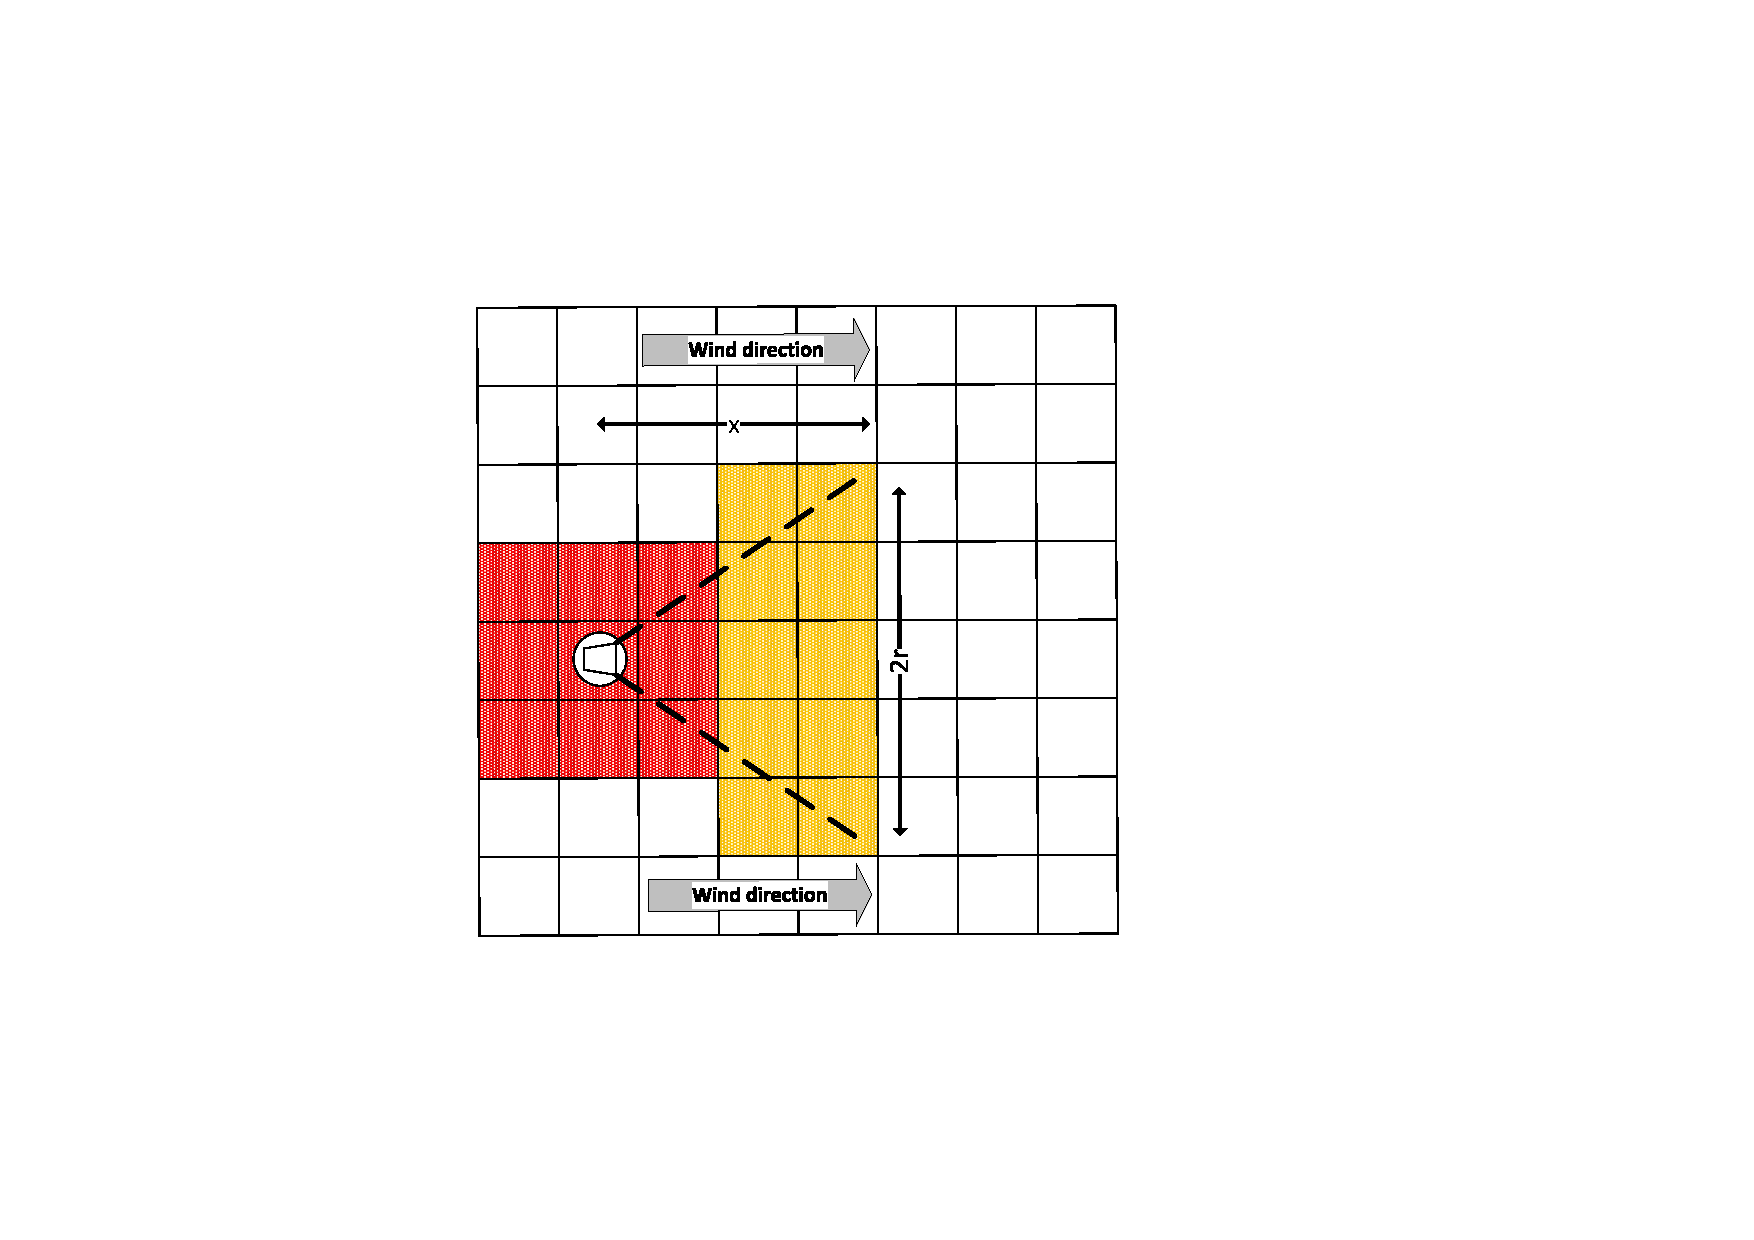
\includegraphics[scale = 0.9]{field_model.pdf}

	\caption{Wind farm model: proximity constraints, wakes, wind direction.}\label{fig:field_model}
\end{figure}



\paragraph{Wind Farm as a Grid} We consider a square shaped wind farm that we model 
as an $n\times n$ grid
with $n$ being the number of cells on each axis. 
The cells have an area of $c^2$ (in squared meters), i.e.,
if $c=100$ meters and $n=20$, the farm area will be $2km\times 2km$.
In this work, we assume that the terrain is flat and that 
we have no constraints related to the terrain.
Furthermore, we do not account for the influence of noise
on the wind farm's surroundings. The wind farm literature treats the more complex
farm models that capture non-flat terrain~\cite{song2015lazy,kuo2016wind}, multi-typed turbines~\cite{feng2017design}, noise effects~\cite{Zhang2014,sorkhabi2016impact,yin2014multi}, and complex objectives (including turbine installation  and maintenance costs)~\cite{lackner2007analytical}.
In this work, we focus on the novel quadratic approach for WFLO, and hence
consider the most abstract wind farm model. Yet, our model can be extended,
in the future, to include 
additional wind farm settings. \todo{perhaps discuss in future work} 
 
Returning to the grid model, we assume that the number of homogeneous turbines to be placed is known 
in advance; we denote the number of turbines by $m$. To place these $m$ turbines, 
we must consider two types of interference effects, namely \emph{proximity constraints} and \emph{wakes}.
In what follows, we explain the two effects using a toy example of placing a single turbine on an 
$8\times8$ grid (see Figure~\ref{fig:field_model}).

\paragraph{Proximity Constraints} Turbines must be placed at least \emph{five rotor diameters} apart. Depending on the cell size, 
	we shall formulate the corresponding constraint as part of the optimization model. For example, assume that a turbine is placed
	in the center of a cell. Then, given a cell size of $c = 100$ meters and a rotor diameter of $40$ meters, 
	we must ensure that two turbines will not placed inside two adjacent cells. In Figure~\ref{fig:field_model}, 
	the red area around the turbine represents the forbidden cells.
	 
\paragraph{Wakes} Turbines influence each other through interference effects that are referred to as \emph{wakes}~\cite{jensen1983note,shakoor2016wake}. 
	 Wakes cause reduction of the effective power produced by a turbine due to upstream turbines that change
	 its airflow dynamics. In Figure~\ref{fig:field_model}, the wind is assumed to be horizontal. Therefore, the wake effect due
	 to placing the turbine expands as shown in the diagram: it will influence only turbines that will be placed in the orange cells.
	 In other words, if a turbine is placed in the orange area, its effective
	 power is reduced due to the upstream turbine that we placed in the $8\times8$ farm. 
	 Moreover, wakes can occur between multiple turbines, and hence
	 multiple wakes must be taken into account for each location. 
	 The reduction of power due to the wake effect is determined by three parameters: (1) the distance between the upstream
	 turbine and the cell for which we want to compute the effect (denoted by $x$ in Figure~\ref{fig:field_model}), (2) the radius of the cone's opening 
	 (denoted by $r$ in Figure~\ref{fig:field_model}), and (3) 
	 the superposition of several wind regimes (a wind regime is a combination of free speed and directions).
	 The wake effect can be pre-computed for each pair of cells 
	 since we know: the distance ($x$), the turbine specifications and terrain conditions (that jointly dictate $r$), and  
	 probabilistic behavior of wind regimes~\cite{Zhang2014}. 
	 
\paragraph{Effective Power Calculations in the Presence of Wakes} 
Let $\mathcal{D}$ be the set of wind regimes. Every regime $d\in \mathcal{D}$ is a unique combination of wind direction and free speed. 
The probability of wind regime 
$d \in \mathcal{D}$ is given by $p_d$ with $\sum_{d \in \mathcal{D}}^{} p_d = 1$. In the experimental section (Section~\ref{sec:eval}),
we provide one example of a probability distribution 
function over $36$ wind regimes (Figure~\ref{fig:prob_wind}). In that example, 
a regime $d=(10deg, 12km/h)$ corresponds to a north-eastern wind blowing at a free velocity of $12km/h$. The
probability of this regime is $0.008$. Let $u_{id}$ be the wind velocity at turbine $i = 1,\ldots, m$ for wind regime $d\in\mathcal{D}$. 
Note that turbines can adjust their direction according to the current wind 
regime. 

Given that we must consider wakes, the velocity $u_{id}$ is not equivalent to the free wind speed of $d$.
The actual velocity at turbine $i$, $u_{id}$, can be computed using the following equation~(\cite{Zhang2014}):
\begin{equation}
u_{id} = u_{id\infty} \Bigg[1 - \sqrt{\sum_{j\in\mathcal{U}_{id}} \bigg( 1-\frac{u_{ijd}}{u_{id\infty}} \bigg)^2}  \Bigg], \label{eq:ss}
\end{equation} with $u_{id\infty}$ being the free wind speed (second component of regime $d$), the set of turbines $\mathcal{U}_{id}$ that are upstream to $i$ 
under wind regime $d$, and $u_{ijd}$ being the wake 
reduced speed at $i$ due to upstream turbine $j$. 
The reduced speed, $u_{ijd}$, is computed using the distance $x$ between the two turbines ($i,j$)  and turbine and terrain specifications that yield the cone opening radius, $r$. Furthermore, the set of upstream turbines, $\mathcal{U}_{id}$ is computed  
by rotating the grid w.r.t. to the current wind regime $d \in \mathcal{D}$ and computing which turbine $j$ is located upstream to turbine $i$ given $d$. The expression in Eq. (\ref{eq:ss}) is referred to as the \emph{sum-of-squares} (SS) model for 
the total expected power in presence of wakes~\cite{Zhang2014}.  We can now write 
the sum-of-squares (SS) expected power of a wind farm with $m$ turbines~(\cite{Zhang2014}): \begin{equation} E_{SS} = \sum_{i=1}^m \sum_{d\in\mathcal{D}} \frac{1}{3} u_{id}^3p_d. \end{equation} This is also known to be the most accurate analytical total power expression that accounts for multiple wakes. However, the expression is not amenable for optimization, and hence, a simplified representation for the total expected energy that considers wakes is required. 

An alternative 
form of the total expected power in the presence of multiple wakes is the linear superposition (LS) expression: \begin{equation} \label{eq:ls}
E_{LS} = \sum_{i=1}^m \sum_{d\in\mathcal{D}} \Bigg(\frac{1}{3}u_{id\infty}^3 -\sum_{j\in\mathcal{U}_{id}} \frac{1}{3}(u_{id\infty}^3 - u_{ijd}^3)\Bigg).
\end{equation} Note that $E_{LS}$ has the same parameters as $E_{SS}$; the difference is in the function that ties these parameters together. 
The LS model is known to be less accurate compared to SS, yet as we will show in Section~\ref{sec:QUBO4WFLO} it 
results in a quadratic objective function in our WFLO formulations, which is a desired property from an optimization standpoint.
 

\subsection{Optimization Methods for WFLO}

The allocation of turbines in a grid-like wind farm was first considered 
as an optimization problem in~\cite{MOSETTI1994105}. The proposed method in~\cite{MOSETTI1994105}
searches for improved solutions using a 
genetic approach~\cite{davis1991handbook},
which is an approximate technique 
that does not aim to provide an optimal solutions;
instead, it attempts to find a quick turbine placement.


In follow-up works, 
the WFLO problem was solved using \emph{exact}  
optimization methodologies~\cite{turner2014new,Zhang2014}. 
These methods guarantee that the returned solution is optimal with respect
to the specified objective (i.e., maximize total expected power). 
Indeed, the exact methods were shown to yield higher energy values, yet they often suffer from 
high computational cost and long runtimes. Therefore, one must strike a balance between optimality and computational requirements of the solution. 
Fast solutions are useful when solving the wind farm design problem numerous times (e.g., when considering different numbers of turbines and various locations),
while optimal solutions yield better placements in terms of the total expected energy.

In what follows, we provide a literature review that covers both approaches, namely exact vs. approximate WFLO.
We subsequently relate our 
work to both exact and approximate methods via our proposed quadratic optimization paradigm for WFLO\footnote{We shall review 
only literature that considers the same wind farm model as the one presented at the beginning of this section}. 
 
\paragraph{Exact Optimization Methods} 
\todo{Rephrase and add citations to exact methods}
The WFLO problem can be solved  
to optimality, using
techniques from operations research (e.g., mixed-integer linear programming (MILP), quadratic programming (QP), and constraint programming (CP))~\cite{}.
These methods are \emph{exact}, in the sense that they guarantee that the returned solution is indeed
the best solution one can obtain for the given problem. Donovan was the first to solve WFLO using a
MILP approach based on the LS energy expression~\cite{donovan2005wind}. In~\cite{turner2014new}, the authors
approximated the SS energy expression using a quadratic and a linear approximation. The two resulting methods performed well
compared to existing approximate and exact methods~\cite{turner2014new}. 

The most recent attempt to solve the wind farm variation that we presented 
in this section is given in~\cite{Zhang2014}. The authors compared
previously existing MILP and QP models to their approach for directly optimizing the SS objective. To this end, they used constraint programming (CP), which 
is an optimization technique that does not make assumptions on the functional form of the objective.
This turned out to be computationally intractable for the larger standard WFLO benchmarks. 

In our work, we build upon the approach in~\cite{donovan2005wind}, yet instead of using a linear version of the LS objective, we 
model WFLO using a more natural quadratic representation. The difference between our approach and the quadratic model
proposed in~\cite{turner2014new} is that our model is not an approximation, but rather an exact representation of the LS objective.

As we mentioned before, the main advantage of exact techniques
is that they provide guarantees on solution quality. However, their disadvantage is
that they may take a very long time to execute before finding an optimal solution. 
In fact, Section~\ref{sec:QUBO4WFLO} shows that WFLO is computationally hard, a result
that we have not yet encountered in the WFLO literature. Therefore,
when one considers solving multiple wind farm design problems, a fast solution is of essence,
and hence one may turn to approximate WFLO.

\paragraph{Approximate Methods} \todo{tighten} In contrast to exact methods, approximation algorithms often provide   
quick and sufficiently accurate solutions. Several works solved 
WFLO using evolutionary (genetic) approaches~\cite{MOSETTI1994105,gonzalez2010optimization,grady2005placement}. 
These methods use two principles (cross-over and mutation)
to change existing solutions and improve them over time. Evolutionary methods do not guarantee termination 
(i.e., they may run forever without achieving a quality criteria), and when they do terminate (in practical cases) they do
not guarantee optimal solutions. Hence, one must often
introduce non-quality related stopping criteria, 
thus compromising on quality of the attained solution~\cite{davis1991handbook}.
Furthermore, there is no natural way of introducing constraints into genetic methods, which
leads to a potentially costly feasibility check for every solution. 

The first attempt to address these limitations 
was made in a local search approach for WFLO~\cite{ozturk2004heuristic}. 
The solution does not guarantee optimality, 
yet it circumvents the termination and feasibility checking issues of the evolutionary
methods. The local search approach attempts to apply either move, remove or add actions given an incumbent 
feasible solution. When a turbine is moved, removed or added, the new solution is evaluated. The procedure terminates 
when a stopping criteria is reached.
The main limitation of~\cite{ozturk2004heuristic} is that it cannot perform an action 
that leads to an infeasible state. Therefore, it quickly converges to a sub-optimal solution (local optimum) 
that can potentially by far
from the globally optimal solution. This problem was experimentally demonstrated in~\cite{rivas2009solving}. 

To overcome this limitation, the authors of~\cite{rivas2009solving} used simulated annealing (SA), 
a neighborhood search method that allows visits to infeasible solutions. 
This creates a well-connected solution space that leads the algorithm to escape 
local optima. The SA method was shown to be superior to~\cite{ozturk2004heuristic} 
and to the genetic method proposed in~\cite{grady2005placement}. A drawback of the SA approach 
is its ad-hoc nature. The various components of the algorithm
 must be tailored and geared towards WFLO. This means that small adjustments to our WFLO setting
 (e.g., adding noise considerations), would require major changes to the SA solution. 
Additional methods and experimental comparisons between various approximate algorithms are available in~\cite{samorani2013wind}.

In our work, we also use an SA approach (similarly to~\cite{rivas2009solving}). However,
our methodology is generic since it is based on our quadratic paradigm and
on the ability of specialized hardware to solve quadratic (non-ad-hoc) models.
Quadratic WFLO models can be easily adjusted to include additional problem features, e.g., wind farm characteristics. 

\paragraph{Quadratic Programming as a Unified Framework for Exact and Approximate WFLO}
\todo{send a clear message here. Perhaps move to next section}.

In this work, we argue that 
formulating WFLO using quadratic programming enables us to employ 
advanced software solutions (e.g., Gurobi optimizer) and approximate hardware developments 
(e.g., Fujitsu's digital annealer that solves quadratic problems using principles from simulated annealing). 
A benchmark study compared state of the art exact approaches from~\cite{Zhang2014} to 
approximate methods and found that the two perform in a comparable fashion, without large differences between
the attained energy~\cite{yang2019simulated}. Exact methods tend to perform slightly better
in smaller WFLO benchmarks, while simulated annealing methods dominated for larger standard WFLO benchmarks. 
This leads to the conclusion that both types of methods (exact and approximate) should be considered. 
Therefore, in this work, we use a unified paradigm that would enable both exact and approximate solutions to WFLO. Thus, 
our approach `enjoys' the best of both worlds. 

%
%
%Specifically, we consider two variations of the quadratic programming paradigm.  
%The first one is referred to as quadratic constrained optimization problems (QCOP). 
%It enables maximizing a quadratic (LS-based) energy expression, while 
%ensuring that WFLO constraints are maintained (turbine proximity and total number of turbines is $m$). 
%The second model is a quadratic unconstrained binary optimization (QUBO), 
%which 
%
%
%On the one hand, exact solvers for quadratic programs (QCOP and QUBO) such as Gurobi~\cite{}, 
%use cutting edge
%operations research methods to enhance performance.
%On the other hand, simulated annealing methods have been recently embedded onto 
%designated processing units. These units use quantum-inspired technology to solve
%complex problems quickly and with minimal degradation in terms of the resulting solution~\cite{}.
%Specifically, in this work, we shall use Fujitsu's digital annealer (DA) to solve WFLO. The DA
%also requires a quadratic representation of the WFLO problem. 
%
%Both of these methods use 
%quadratic optimization models, which we shall present in the next section (Section~\ref{sec:QUBO4WFLO}).
%


\section{Quadratic Models for WFLO}
\label{sec:QUBO4WFLO}

In this part, 
we formulate the WFLO problem
using quadratic programming. Specifically, we consider two
quadratic optimization problems that represent WFLO: a
quadratic constrained optimization (QCOP) problem and 
a quadratic unconstrained binary optimization (QUBO) problem. 
The former represents WFLO characteristics (proximity and number of turbines)
as hard constraints, while the latter considers these characteristics as soft constraints that are added to its objective function.

We start by presenting the inputs and decision variables into our optimization approaches.
Subsequently, we introduce the two quadratic formulations of WFLO and 
prove its computational complexity. Lastly, we discuss the details of existing
software and hardware solutions that can be used to solve the two formulations. 

\subsection{WFLO Inputs and Decision Variables} We consider the wind farm model that we presented in Section~\ref{sec:related}. 
Let $x_i$ be a binary decision variable that represents whether a 
turbine is positioned at location 
$i \in \mathcal{N}$ with $\mathcal{N}$ being the set 
of $k = n^2$ possible turbine locations (cells in the grid). We 
write $x$ as shorthand for $x = (x_1,\ldots, x_k)$. Furthermore,
we denote by $\mathcal{E} \subseteq \mathcal{N}\times \mathcal{N}$
the set of location pairs that cannot simultaneously host turbines 
due to proximity constraints. The set $\mathcal{E}$ can be pre-computed 
based on problem specifications. For example,
it is common to assume that two turbines must be placed at least five rotor diameters apart. 

Let $u_{id}$ and $u_{id\infty}$ 
be the wind speeds at turbine location $i \in \mathcal{N}$ for wind regime $d \in \mathcal{D}$
with and without interference from other turbines due to wake effects, respectively. 
Note that here we refer to $i$ as a potential turbine location and not the $i$th turbine as we did in Section~\ref{sec:related}.
Further, we denote by $\mathcal{U}_{id} \subseteq \mathcal{N}$ 
the set of upstream 
turbine locations for wind regime $d$
given that a turbine is placed at cell $i$ (i.e., turbines placed in these locations 
will be influenced by a turbine placed in $i$). Finally,
we denote by $u_{ijd}$ the wind speed at location $j$ due to a single wake from upstream turbine at location $i$ with $j \in \mathcal{U}_{id}$. 
The following function  
represents the total expected energy of a wind farm given placement decisions 
$x$: \begin{equation}
f(x) = \sum_{i \in \mathcal{N}}^{} \sum_{d \in \mathcal{D}}^{} p_d ( \frac{1}{3} \ u_{id, \infty}^3 x_i  - \sum_{j \in \mathcal{U}_{id}}^{} \frac{1}{3}(u_{id, \infty} ^3 - u_{ijd}^3)x_i x_j).   \label{ObjFunc}\\
%&s.t.:& \nonumber\\
%&\mbox{       }& \sum_{i \in \mathcal{N}}^{} x_i = m,\label{Cardinality}\\
%&\mbox{       }& x_i + x_j \leq 1,   \forall (i,j) \in \mathcal{E}, \label{Grid}\\
%&\mbox{       }& x_i \in \{0,1\},     \forall i \in \mathcal{N}.
\end{equation} The objective function corresponds to the linear superposition (LS)
expression (Eq.~\ref{eq:ls}). We are now ready to provide the two quadratic programs to represent WFLO.

\subsection{WFLO as QCOP}

To 
maximize $f(x)$ and satisfy the total number of turbines and proximity 
constraints we write
the following quadratic optimization problem (QCOP):
\begin{eqnarray} \label{QCOP}
&\max_{x_i}^{}& \sum_{i \in \mathcal{N}}^{} \sum_{d \in \mathcal{D}}^{} p_d ( \frac{1}{3} \ u_{id, \infty}^3 x_i  - \sum_{j \in \mathcal{U}_{id}}^{} \frac{1}{3}(u_{id, \infty} ^3 - u_{ijd}^3)x_i x_j)   \\
&s.t.:& \nonumber\\
&\mbox{       }& \sum_{i \in \mathcal{N}}^{} x_i = m,\label{Cardinality}\\
&\mbox{       }& x_i + x_j \leq 1,   \forall (i,j) \in \mathcal{E}, \label{Grid}\\
&\mbox{       }& x_i \in \{0,1\},     \forall i \in \mathcal{N}.
\end{eqnarray} Constraint~\ref{Cardinality} and \ref{Grid} ensure that exactly $m$ turbines are placed on the grid
and enforce proximity constraints between the turbines, respectively. 

The QCOP presented as Problem~\ref{QCOP} can be solved using an exact optimization solver, e.g., Gurobi~\cite{gurobi}. 
So far, in~\cite{Zhang2014} and~\cite{donovan2005wind}, equivalent (linear) problems were formulated and solved using 
exact solvers. However, these solvers should only be used if the problem is computationally hard.
We are unaware of an existing complexity result for the LS variation in Eq.~\ref{QCOP}. In what follows, we provide
a theorem that proves the computational complexity of WFLO. 
\begin{mythm}
	The computational complexity of WFLO is $\mathcal{NP}$-hard. 
\end{mythm}
\begin{myproof}
We prove by showing that a special case of the WFLO problem (Eq.~(\ref{QCOP}) is
$\mathcal{NP}$-hard. Suppose that $\mathcal{E} = \emptyset$, i.e., the grid is coarse grained enough to ignore proximity constraints. Then, the constraints in Eq.~(\ref{Grid})
are dropped and we get the heaviest k-subgraph problem (HSP), which was proven to be $\mathcal{NP}$-hard in~\cite{billionnet2005different}.
Since a special case of WFLO is  $\mathcal{NP}$-hard it implies that WFLO is at least $\mathcal{NP}$-hard. On the other hand,
WFLO is formulated using integer programming (Problem \ref{QCOP}), which means that it is at most $\mathcal{NP}$-hard. Therefore, we get that WFLO is $\mathcal{NP}$-hard.
	\end{myproof} To overcome the challenge associated with the computational hardness of WFLO,
we reformulate the QCOP into a QUBO problem.  


\subsection{WFLO as QUBO}

Quadratic unconstrained binary optimization problems, as their name implies, cannot have constraints. Alternatively, they only 
have an objective function that 
one can to maximize (or minimize). Furthermore, the decision variables must be binary. Let $\lambda = (\lambda_1,\lambda_2)$ 
be a vector of constraint parameters with $\lambda_i >0$. The equivalent QUBO formulation of the QCOP in Eq.(\ref{QCOP}) is given by,
\begin{equation}\max_{x}^{} f(x) - \lambda_1 (\sum_{i \in \mathcal{N}}^{} x_i -m) ^2 - \lambda_2 \sum_{(i,j) \in \mathcal{E}}^{} x_i x_j , \label{QUBO}\end{equation}
with the term $ \lambda_1 (\sum_{i \in \mathcal{N}}^{} x_i -m) ^2$ 
penalizing solutions that violate the exactly $m$ turbines constraint, while the term $\lambda_2 \sum_{(i,j) \in \mathcal{E}}^{} x_i x_j$ penalizes
solutions that place turbines in high proximity. The two penalty terms $\lambda_1$ and $\lambda_2$ 
must be large enough to ensure that the solutions are indeed feasible. These types of constraints
are referred to as \emph{soft constraints} as they do not guarantee a feasible solution 
for an arbitrary selection of $\lambda$.   


\subsection{Solving QCOP and QUBO using Advanced Optimization Methods}

\subsubsection{QCOP solving methods}

\todo{Jason's part}

\subsubsection{Specialized Hardware for QUBO}

\todo{Eldan's part}


\section{Evaluation}
\label{sec:eval}

In this section, we 
present an empirical evaluation of our quadratic models based on 
standard WFLO instances.
Our main results are: \begin{itemize}
	\item QUBO based WFLO using the digital annealer provides state-of-the-art results in seconds.
	\item Given enough time LS quadratic models are superior to both linear models and to an SS approximations. 
\end{itemize}
We start by outlining the experimental design of our evaluation, followed by a presentation of our main results
and a discussion of the results together with the limitations of the approach.

\subsection{Experimental Design}



\paragraph{WFLO Instances}
\begin{figure}[t]
	\centering
	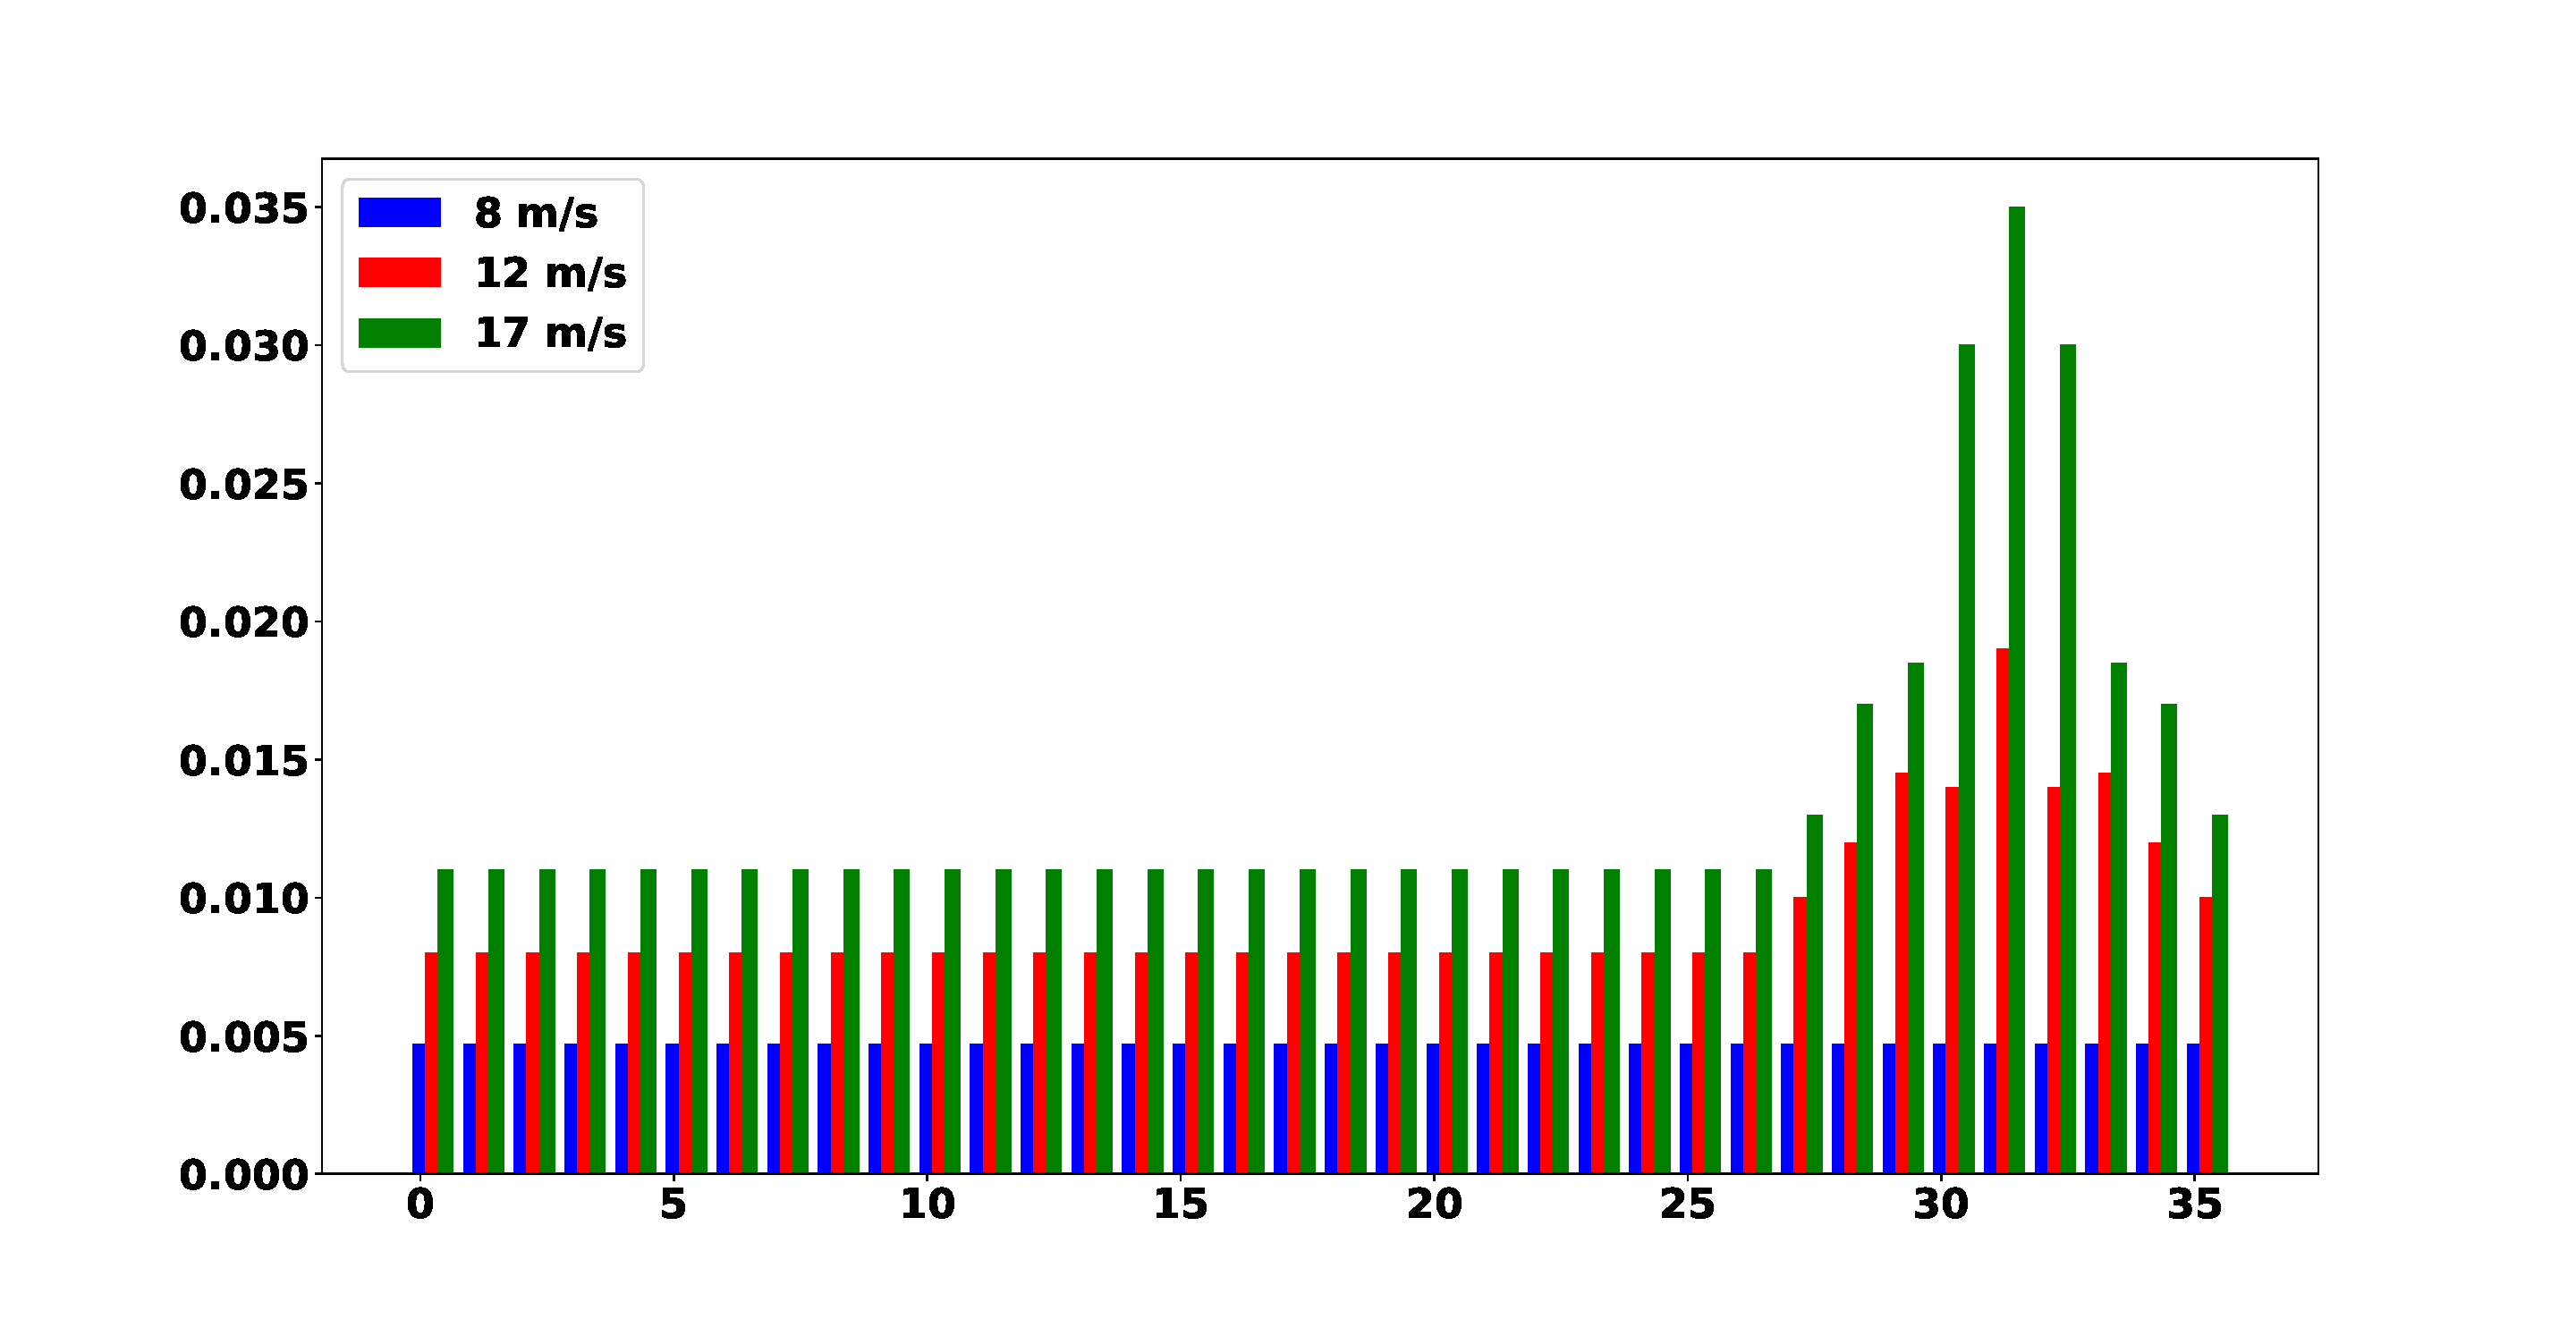
\includegraphics[scale = 0.3]{prob_wind_pdf.pdf}
	
	\caption{Wind regimes: x-axis is the angle (times 10 degrees), y-axis is the probability for wind regime, color corresponds to free wind speed.}\label{fig:prob_wind}
\end{figure}

\paragraph{Optimization Benchmarks}

\paragraph{Experimental Setting}

\paragraph{Implementation Details}


\subsection{Main Results}

\begin{table}[ht]

	\begin{tabular}{| c | c | c | c | c | c | c | c |}
		\toprule
		Wind Directions  & n        & m        & ILP-LS       & QP-LS       & QUBO-LS       & QP-SS       & DA-LS     \\
		\toprule
		\multirow{6}{*}{WR1}  & \multirow{3}{*}{10}       & 20       & \textbf{11185.41} & \textbf{11185.41} & \textbf{11185.41} & \textbf{11185.41} & \textbf{11185.41} \\
			& & 30   & 15739.57 & 15738.45 & \textbf{15742.93} & 15735.1  & 15740.69         \\
		& & 40 & \textbf{19265.21} & \textbf{19265.21} & 18952.97 & \textbf{19265.21} & \textbf{19265.21}                \\
				\cline{2-8}
		&\multirow{3}{*}{20}   & 20       & \textbf{11404.8}  & \textbf{11404.8}  & \textbf{11404.8}  & \textbf{11404.8}  & \textbf{11404.8}           \\
		&&30   & \textbf{16770.2} & 16758.45 & 16715.19 & 16755.75 & 16570.96                   \\
		&&40   & \textbf{21977.17} & 21963.8 & 21643.56 & \textbf{21977.17} & 21874.04                     \\
		\hline
		\multirow{6}{*}{WR36} &  \multirow{3}{*}{10}    & 20       & 19022.77 & \textbf{19221.44} & \textbf{19221.44} & 19193.42 & \textbf{19221.44} \\
		&& 30   & 27247.5  & 27442.9  & 27418.74 & 27387.06 & \textbf{27450.99}                  \\
		&&40   & 34671.62 & \textbf{34938.65} & \textbf{34938.65} & 34817.27 & 34888.81                  \\
		\cline{2-8}
		&  \multirow{3}{*}{20}   & 20       & 18448.64 & 19336.33 & 19172.56 & 19354.23 & \textbf{19441.17}          \\
		&&30   & 26367.2  & 27752 & 27785 & 27492.11 & \textbf{27975.55}                     \\
		&&40   & 33451.94 & \textbf{35665.6}  & 35127.32 & 35065.85 & 35604.45  \\
		\bottomrule                   
	\end{tabular}

\vspace{0.5em}
\caption{Total Expected Power (kilo Watt/year) after 3600 seconds as function of benchmark and method}\label{tab:results1}
\end{table}



\begin{figure}[t!]%
	
	\subfloat[MRE after 50 seconds]{{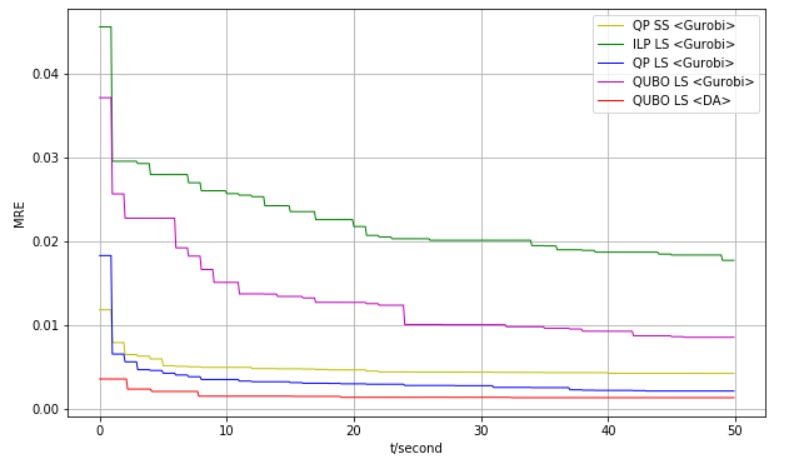
\includegraphics[width=0.5\textwidth]{energy_50.png} }}%
	\quad
	\subfloat[MRE after 1 hour]{{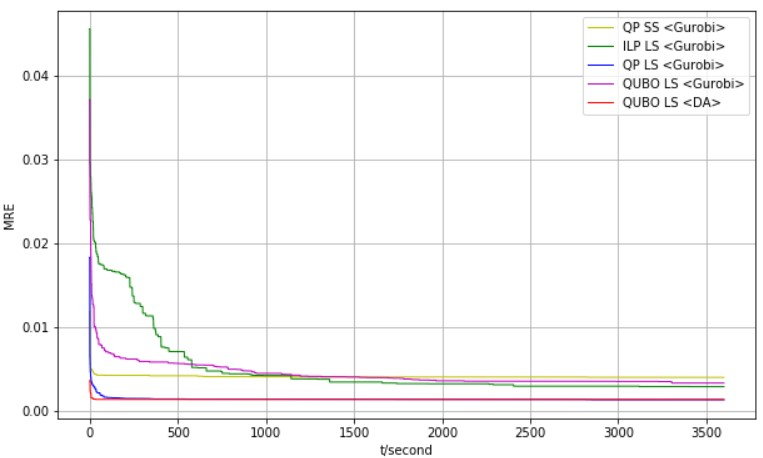
\includegraphics[width=0.5\textwidth]{energy_3600.png} }}\\%\\
	\caption{Mean Relative Energy (w.r.t. best feasible solution) vs. Runtime.}%
	
	\label{fig:main_effects}%
\end{figure}

\subsection{Discussion \& Limitations}



\section{Conclusion}
\label{sec:conclusion}

\bibliographystyle{elsarticle-num-names}
%\bibliographystyle{plainnat}
\bibliography{Biblio}

\end{document}



%
%\begin{table}[t]
%	
%
%	\label{tab:results1}
%	\vspace{-0.5em}
%	\scriptsize
%	\centering
%	\begin{tabular}{ c @{\hspace{1em}} c @{\hspace{1em}} c @{\hspace{1em}} c}
%		\toprule
%		Paper & Exact Optimization & Discrete Grid & Flat Terrain  \\
%		\midrule
%		\citet{Zhang2014,turner2014new} & + & + & +  \\
%		\citet{kuo2016wind} & + & + & -  \\
%		 \citet{} & + & - & + \\
%		
%		\bottomrule
%	\end{tabular}
%	\vspace{-1em}
%	\caption{Literature review of Wind Farm Optimization Layout solutions.}
%		
%\end{table}

